\documentclass[12pt]{article}
\usepackage[utf8]{inputenc}
\usepackage[spanish]{babel}
\usepackage{amsmath}
\usepackage{amsthm}
\usepackage{amssymb}
\usepackage{fancyhdr}
\usepackage{mathpazo,amsfonts}
\usepackage[margin=0.95in]{geometry}
\usepackage{tikz}


\usepackage[
backend=biber,
style=alphabetic,
sorting=ynt
]{biblatex}

\addbibresource{blb.bib}

\pagestyle{fancy}

\lhead{Tarea 2}
\chead{Luis González}
\rhead{4 de marzo de 2022}

\newcommand{\N}{\mathbb{N}}
\newcommand{\Z}{\mathbb{Z}}
\newcommand{\Q}{\mathbb{Q}}
\newcommand{\R}{\mathbb{R}}

\newtheorem{prop}[section]{Proposición}

\newenvironment{problem}[2][Problema]{\begin{trivlist}
\item[\hskip \labelsep {\bfseries #1}\hskip \labelsep {\bfseries #2.}]}{\end{trivlist}}

\begin{document}
\section*{Teoría de Gráficas}


%---------------------------------------
\begin{problem}{1.5.3} \text{ } 
\begin{itemize}
    \item[a)] Demuestre que los cuatro torneos descritos en la Figura \ref{fig:fig1} son no isomorfos por parejas, y que estos son únicos en cuatro vértices, salvo isomorfismo.
    \item[b)] ¿Cuántos torneos existen en cinco vértices, salvo isomorfismo?
\end{itemize}
\end{problem}
\begin{proof}\text{}
\begin{itemize}
    \item[a)] Nos referiremos a las digráficas descritas en la Figura \ref{fig:fig1} como $G_1, G_2, G_3$ y $G_4$, procediendo de izquierda a derecha.
    \begin{itemize}
        \item Note que todos los vértices de $G_1$ tienen grado de salida menor que tres, mientras que en $G_2$ su vértice central tiene grado de salida igual a tres. Por tanto $G_1$ y $G_2$ no son isomorfas. 
        \item En la digráfica $G_3$, el vértice central tiene grado de entrada igual a tres, mientras que en $G_1$, todos sus vértices tienen grado de entrada menor que que tres. Por tanto $G_1$ y $G_3$ no son isomorfas.
        \item El vértice superior (ver Figura \ref{fig:fig1}) de la digráfica $G_4$ tiene grado de salida igual a tres, mientras que ningún vértice en $G_1$ satisface esto. Por tanto $G_1$ y $G_4$ no son isomorfas.
        \item El vértice central de la digráfica $G_3$ tiene grado de entrada igual a tres. Todo vértice de $G_2$ tiene grado de entrada igual a dos. Por tanto $G_2$ y $G_3$ no son isomorfas.
        \item El vértice central de la digráfica $G_4$ tiene grado de entrada igual a uno, mientras que ningún vértice de $G_2$ satisface lo anterior. Por tanto $G_2$ y $G_4$ no son isomorfas. 
        \item Finalmente, note que el vértice superior de la digráfica $G_4$ tiene grado de salida igual a tres. Todo vértice de $G_3$ tiene grado de salida menor que tres. Por lo que $G_3$ y $G_4$ no son isomorfas.
    \end{itemize}
    
    Note que estos son los únicos torneos en cuatro vértices, salvo isomorfismo. Para ver esto, note que, si cambiamos la orientación de una arista de la $G_i$, entonces obtenemos otra gráfica $G_j$ ($i \neq j$) que aparece en la Figura 1.
    
    \item[b)] Existen 12 torneos en  cinco vértices, salvo isomorfismo, como se muestra en la sucesión A000568 de \cite{oeis}.
\end{itemize}
 
\end{proof}
%---------------------------------------
\begin{figure}[h]
    \centering
    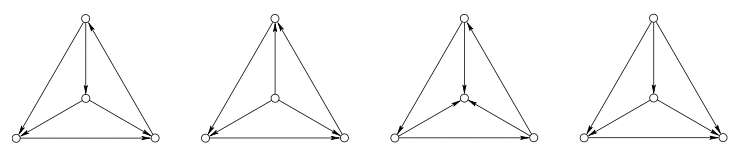
\includegraphics[scale=0.60]{pics/graph3.png}
    \caption{Torneos en cuatro vértices}
    \label{fig:fig1}
\end{figure}

\newpage
%---------------------------------------
\begin{problem}{2.1.2} \text{ }
\begin{itemize}
    \item[a)] Demuestre que toda gráfica no trivial acíclica tiene al menos dos vértices de grado menor que dos.
    \item[b)] Deduzca que toda gráfica no trivial, acíclica y conexa tiene al menos dos vértices de grado uno. ¿Bajo qué condiciones se satisface la igualdad?
\end{itemize}
\end{problem}
\begin{proof}
\text{}
\begin{itemize}
    \item[a)] Se procederá por inducción en el número de vértices de $G.$ Si $G$ es acíclica en tres vértices, entonces $G$ es una trayectoria, o $G$ tiene un vértice aislado. En ambos casos $G$ tiene dos vértices de grado menor que dos. 
    
    Ahora suponga que la proposición es cierta para toda gráfica acíclica con menos de $n \geq 3$ vértices. Sea $G$ una gráfica acíclica en $n$ vértices. Por el \textbf{Teorema 2.1} de \cite{10.5555/1481153}, $G$ tiene un vérice $u$ de grado menor que dos. Considere la gráfica $H = G - u$. Note que $H$ es acíclica, pues de lo contrario $G$ tendría un ciclo (contenido en $H$). Como $H$ tiene menos de $n$ vértices, la hipótesis de inducción implica que $H$ tiene dos vértices $v, w$ de grado menor que dos. A lo más uno de estos, digamos $v$, es adyacente a $u$ en $G$, pues $u$ es de grado menor que dos. Luego, $w$ también es de grado menor que dos en $G$, demostrando lo que se quería.
    
    
    \item[b)] Sea $G$ una gráfica acíclica y conexa. Note que el argumento descrito en a) aplica para este caso, pues no asumimos conexidad. Por tanto, $G$ tiene dos vértices $u,v$  de grado menor que dos. Sin embargo, la conexidad implica que todo vértice de $G$ tiene grado mayor a cero. Por tanto $u,v$ tiene grado uno en $G.$
    
    
    Se demostrará por inducción en el número de vértices, que si $G$ es acíclica, conexa y con únicamente dos vértices de grado uno, entonces $G$ es una trayectoria. Si $G$ es una gráfica en dos vértices, entonces como estos tienen grado uno, estos son adyacentes. Luego $G$ es una trayectoria. 
    
    Ahora suponga que la proposición es cierta para toda gráfica acíclica, conexa, con solo dos vértices de grado uno y con menos vértices que $n \geq 2.$ Sea $G$ una gráfica en $n$ vértices que satisface las anteriores condiciones. Sean $u,v$ los vértices de $G$ de grado uno y sea $H = G \setminus \{u,v\}.$ Note que $H$ es acíclica y como tanto $u$ como $v$ son de grado uno, $H$ es conexa. Entonces la hipótesis de inducción establece que $H$ es una trayectoria. Luego, existen vértices $w,z$ en $H$ con grado uno. Observe que $w,z$ son de grado dos en $G$, pues de lo contrario $G$ tendría más de dos vértices de grado uno. Lo anterior implica que $u$ es adyacente a $w$ y $v$ es adyacente a $z$ en $G$; o bien, $u$ es adyacente a $z$ y $v$ es adyacente a $w$ en $G.$ Pero como $H$ es una trayectoria, lo anterior implica que $G$ también lo es.

   
\end{itemize}
\end{proof}
%---------------------------------------

%---------------------------------------
\begin{problem}{2.1.11}\text{}
\begin{itemize}
    \item[a)] Demuestre que toda digráfica acíclica tiene al menos una fuente y un pozo. 
    \item[b)] Deduzca que una digráfica admite un ordenamiento topológico si y solo si es acíclica. 
\end{itemize}
\end{problem}
\begin{proof}\textbf{ }
\begin{itemize}
    \item[a)] Sea $D$ una digráfica acíclica en $n$ vértices. Se demostrará que si $D$ no tiene pozo o fuente, entonces $D$ contiene un ciclo dirigido. Suponga que $D$ no tiene un pozo (si $D$ no tiene fuente, se procede de manera similar). Entonces si $v$ es un vértice de $D$, existe un vértice $u$ que es adyacente a $u$,  mediante una arco  $(u,v).$ De esta manera, podemos seleccionar $v_1, v_2, \ldots, v_{n+1}$ vértices de $D$, con $(v_i, v_{i+1}) \in A(D).$ Como $D$ tiene $n$ vértices, por el Principio del Palomar se deduce que $v_i = v_j$, con $i < j.$ Luego, $v_i v_{i+1} \cdots v_j$ forman un ciclo dirigido en $D.$
    
    
    \item[b)] En lo siguiente, se asume que $D$ es una digráfica conexa. Suponga que $D$ tiene un ordenamiento topológico y suponga que $D$ tiene un ciclo dirigido $C$. Sean $u$, $v$ vértices consecutivos en $C$; esto es, $(u, v) \in A(D).$ Esto implica que $u$ precede a $v$ en el ordenamiento topológico. Por otro lado, como $u, v$ pertenecen al ciclo $C$, existe una trayectoria dirigida $W = u \ldots v$ en $C.$ Luego, $u$ precede a $v$ en el ordenamiento topológico, lo cual es una contradicción. Por tanto $D$ no tiene ciclos.
    
    
    Sean $v_i, v_j, v_k$ tres vértices consecutivos en el ciclo $C.$ Es decir, $(v_i, v_j), (v_j, v_k) \in A(D).$
    
    
    La otra implicación se demostrará por inducción en el número de vértices. Sea $D$ una digráfica acíclica con tres vértices. En la Figura \ref{fig:d3}, se aprecian todas las gráficas acíclicas en tres vértices. Es claro, que las podemos ordenar topológicamente.
    
    Asuma que la proposición es cierta para toda digráfica acíclica con menos vértices que $n\geq3.$ Sea $D$ una digráfica acíclica con $n$ vértices. Por el inciso a), $D$ tiene un pozo $v$. Note que la gráfica $D \setminus v$ es acíclica, pues de lo contrario el ciclo en $D \setminus v$ también sería ciclo en $D$, lo cual contradice el hecho de que $D$ es acíclica. Como $D\setminus v$ tiene menos de $n$ vértices, la hipótesis de inducción establece que  $D\setminus v$ tiene un ordenamiento topológico $(v_1, \ldots, v_{n-1}).$ Luego, la n-tupla $(v_1, \ldots, v_{n-1}, v_n)$ es un ordenamiento topológico de $D$, pues $v$ es un pozo. Por el principio de inducción, se concluye que toda digráfica acíclica tiene un ordenamiento topológico.
    
\end{itemize}
\end{proof}

\begin{figure}
    \centering

\tikzset{every picture/.style={line width=0.75pt}} %set default line width to 0.75pt        

\begin{tikzpicture}[x=0.75pt,y=0.75pt,yscale=-1,xscale=1]
%uncomment if require: \path (0,532); %set diagram left start at 0, and has height of 532

%Straight Lines [id:da7569650426276425] 
\draw    (502.5,213) -- (542.78,140.75) ;
\draw [shift={(543.75,139)}, rotate = 119.14] [color={rgb, 255:red, 0; green, 0; blue, 0 }  ][line width=0.75]    (10.93,-3.29) .. controls (6.95,-1.4) and (3.31,-0.3) .. (0,0) .. controls (3.31,0.3) and (6.95,1.4) .. (10.93,3.29)   ;
%Straight Lines [id:da005055592575455514] 
\draw    (502.5,213) -- (583,213) ;
\draw [shift={(585,213)}, rotate = 180] [color={rgb, 255:red, 0; green, 0; blue, 0 }  ][line width=0.75]    (10.93,-3.29) .. controls (6.95,-1.4) and (3.31,-0.3) .. (0,0) .. controls (3.31,0.3) and (6.95,1.4) .. (10.93,3.29)   ;
%Straight Lines [id:da9679509522489633] 
\draw    (543.75,139) -- (584.03,211.25) ;
\draw [shift={(585,213)}, rotate = 240.86] [color={rgb, 255:red, 0; green, 0; blue, 0 }  ][line width=0.75]    (10.93,-3.29) .. controls (6.95,-1.4) and (3.31,-0.3) .. (0,0) .. controls (3.31,0.3) and (6.95,1.4) .. (10.93,3.29)   ;
%Shape: Circle [id:dp7867827232385834] 
\draw  [fill={rgb, 255:red, 255; green, 255; blue, 255 }  ,fill opacity=1 ] (540.75,139) .. controls (540.75,137.34) and (542.09,136) .. (543.75,136) .. controls (545.41,136) and (546.75,137.34) .. (546.75,139) .. controls (546.75,140.66) and (545.41,142) .. (543.75,142) .. controls (542.09,142) and (540.75,140.66) .. (540.75,139) -- cycle ;
%Shape: Circle [id:dp6276313366796464] 
\draw  [fill={rgb, 255:red, 255; green, 255; blue, 255 }  ,fill opacity=1 ] (582,213) .. controls (582,211.34) and (583.34,210) .. (585,210) .. controls (586.66,210) and (588,211.34) .. (588,213) .. controls (588,214.66) and (586.66,216) .. (585,216) .. controls (583.34,216) and (582,214.66) .. (582,213) -- cycle ;
%Shape: Circle [id:dp007504510445030199] 
\draw  [fill={rgb, 255:red, 255; green, 255; blue, 255 }  ,fill opacity=1 ] (499.5,213) .. controls (499.5,211.34) and (500.84,210) .. (502.5,210) .. controls (504.16,210) and (505.5,211.34) .. (505.5,213) .. controls (505.5,214.66) and (504.16,216) .. (502.5,216) .. controls (500.84,216) and (499.5,214.66) .. (499.5,213) -- cycle ;
%Straight Lines [id:da5855072031840134] 
\draw    (371.5,213) -- (411.78,140.75) ;
\draw [shift={(412.75,139)}, rotate = 119.14] [color={rgb, 255:red, 0; green, 0; blue, 0 }  ][line width=0.75]    (10.93,-3.29) .. controls (6.95,-1.4) and (3.31,-0.3) .. (0,0) .. controls (3.31,0.3) and (6.95,1.4) .. (10.93,3.29)   ;
%Straight Lines [id:da7822521124528533] 
\draw    (371.5,213) -- (452,213) ;
\draw [shift={(454,213)}, rotate = 180] [color={rgb, 255:red, 0; green, 0; blue, 0 }  ][line width=0.75]    (10.93,-3.29) .. controls (6.95,-1.4) and (3.31,-0.3) .. (0,0) .. controls (3.31,0.3) and (6.95,1.4) .. (10.93,3.29)   ;
%Shape: Circle [id:dp8136621981305091] 
\draw  [fill={rgb, 255:red, 255; green, 255; blue, 255 }  ,fill opacity=1 ] (409.75,139) .. controls (409.75,137.34) and (411.09,136) .. (412.75,136) .. controls (414.41,136) and (415.75,137.34) .. (415.75,139) .. controls (415.75,140.66) and (414.41,142) .. (412.75,142) .. controls (411.09,142) and (409.75,140.66) .. (409.75,139) -- cycle ;
%Shape: Circle [id:dp2215493963263795] 
\draw  [fill={rgb, 255:red, 255; green, 255; blue, 255 }  ,fill opacity=1 ] (451,213) .. controls (451,211.34) and (452.34,210) .. (454,210) .. controls (455.66,210) and (457,211.34) .. (457,213) .. controls (457,214.66) and (455.66,216) .. (454,216) .. controls (452.34,216) and (451,214.66) .. (451,213) -- cycle ;
%Shape: Circle [id:dp1184688538958083] 
\draw  [fill={rgb, 255:red, 255; green, 255; blue, 255 }  ,fill opacity=1 ] (368.5,213) .. controls (368.5,211.34) and (369.84,210) .. (371.5,210) .. controls (373.16,210) and (374.5,211.34) .. (374.5,213) .. controls (374.5,214.66) and (373.16,216) .. (371.5,216) .. controls (369.84,216) and (368.5,214.66) .. (368.5,213) -- cycle ;
%Straight Lines [id:da1633951029673174] 
\draw    (242.5,213) -- (282.78,140.75) ;
\draw [shift={(283.75,139)}, rotate = 119.14] [color={rgb, 255:red, 0; green, 0; blue, 0 }  ][line width=0.75]    (10.93,-3.29) .. controls (6.95,-1.4) and (3.31,-0.3) .. (0,0) .. controls (3.31,0.3) and (6.95,1.4) .. (10.93,3.29)   ;
%Straight Lines [id:da6241871950319411] 
\draw    (322,213) -- (244.5,213) ;
\draw [shift={(242.5,213)}, rotate = 360] [color={rgb, 255:red, 0; green, 0; blue, 0 }  ][line width=0.75]    (10.93,-3.29) .. controls (6.95,-1.4) and (3.31,-0.3) .. (0,0) .. controls (3.31,0.3) and (6.95,1.4) .. (10.93,3.29)   ;
%Shape: Circle [id:dp45100196620976696] 
\draw  [fill={rgb, 255:red, 255; green, 255; blue, 255 }  ,fill opacity=1 ] (280.75,139) .. controls (280.75,137.34) and (282.09,136) .. (283.75,136) .. controls (285.41,136) and (286.75,137.34) .. (286.75,139) .. controls (286.75,140.66) and (285.41,142) .. (283.75,142) .. controls (282.09,142) and (280.75,140.66) .. (280.75,139) -- cycle ;
%Shape: Circle [id:dp12281437397644135] 
\draw  [fill={rgb, 255:red, 255; green, 255; blue, 255 }  ,fill opacity=1 ] (322,213) .. controls (322,211.34) and (323.34,210) .. (325,210) .. controls (326.66,210) and (328,211.34) .. (328,213) .. controls (328,214.66) and (326.66,216) .. (325,216) .. controls (323.34,216) and (322,214.66) .. (322,213) -- cycle ;
%Shape: Circle [id:dp11958815016064528] 
\draw  [fill={rgb, 255:red, 255; green, 255; blue, 255 }  ,fill opacity=1 ] (239.5,213) .. controls (239.5,211.34) and (240.84,210) .. (242.5,210) .. controls (244.16,210) and (245.5,211.34) .. (245.5,213) .. controls (245.5,214.66) and (244.16,216) .. (242.5,216) .. controls (240.84,216) and (239.5,214.66) .. (239.5,213) -- cycle ;
%Straight Lines [id:da8375379095360066] 
\draw    (191,213) -- (113.5,213) ;
\draw [shift={(111.5,213)}, rotate = 360] [color={rgb, 255:red, 0; green, 0; blue, 0 }  ][line width=0.75]    (10.93,-3.29) .. controls (6.95,-1.4) and (3.31,-0.3) .. (0,0) .. controls (3.31,0.3) and (6.95,1.4) .. (10.93,3.29)   ;
%Shape: Circle [id:dp7368569157560452] 
\draw  [fill={rgb, 255:red, 255; green, 255; blue, 255 }  ,fill opacity=1 ] (191,213) .. controls (191,211.34) and (192.34,210) .. (194,210) .. controls (195.66,210) and (197,211.34) .. (197,213) .. controls (197,214.66) and (195.66,216) .. (194,216) .. controls (192.34,216) and (191,214.66) .. (191,213) -- cycle ;
%Straight Lines [id:da5752399255597169] 
\draw    (152.75,139) -- (112.47,211.25) ;
\draw [shift={(111.5,213)}, rotate = 299.14] [color={rgb, 255:red, 0; green, 0; blue, 0 }  ][line width=0.75]    (10.93,-3.29) .. controls (6.95,-1.4) and (3.31,-0.3) .. (0,0) .. controls (3.31,0.3) and (6.95,1.4) .. (10.93,3.29)   ;
%Shape: Circle [id:dp712954285737623] 
\draw  [fill={rgb, 255:red, 255; green, 255; blue, 255 }  ,fill opacity=1 ] (108.5,213) .. controls (108.5,211.34) and (109.84,210) .. (111.5,210) .. controls (113.16,210) and (114.5,211.34) .. (114.5,213) .. controls (114.5,214.66) and (113.16,216) .. (111.5,216) .. controls (109.84,216) and (108.5,214.66) .. (108.5,213) -- cycle ;
%Shape: Circle [id:dp2635320585560371] 
\draw  [fill={rgb, 255:red, 255; green, 255; blue, 255 }  ,fill opacity=1 ] (149.75,139) .. controls (149.75,137.34) and (151.09,136) .. (152.75,136) .. controls (154.41,136) and (155.75,137.34) .. (155.75,139) .. controls (155.75,140.66) and (154.41,142) .. (152.75,142) .. controls (151.09,142) and (149.75,140.66) .. (149.75,139) -- cycle ;
\end{tikzpicture}
    \caption{Digráficas en tres vértices acíclicas.}
    \label{fig:d3}
\end{figure}

%---------------------------------------

\newpage
%---------------------------------------
\begin{problem}{2.1.12}
Demuestre que toda digráfica acíclica estricta contiene un arco cuyo \textit{reversal} resulta en una digráfica acíclica. 
\end{problem}
\begin{proof}
Sea $D$ una digráfica acíclica. Por el \textbf{Problema 2.1.11}, $D$ tiene un ordenamiento topológico. Esoja un ordenamiento topológico $(v_1, \ldots, v_n)$ de tal manera que todo vértice aislado (en caso de exisitir) en $D$ se encuentra al final del ordenamiento. Sea $k$ el natural mínimo tal que $(v_k, v_{k+1})$ es un arco en $D.$ Sea $D^\prime$ la digráfica obtenida de $D$ cambiando únicamente el arco $(v_k, v_{k+1})$ por el arco $(v_{k+1}, v_{k})$. Considere la permutación $t^\prime$ de  $(v_1, \ldots, v_n)$, definida por la transposición $\tau = (k \ k+1 )$, es decir, 
$$ t^\prime = (v_{\tau(1)}, \ldots, v_{\tau(n)} ).$$ Es claro que $t^\prime$ es un ordenamiento topológico de $D^\prime.$ Por tanto $D^\prime$ es acíclica, que es lo que se quería demostrar. 
\end{proof}
%---------------------------------------



%---------------------------------------
\begin{problem}{2.1.17} Sea $G$ una gráfica simple y libre de triángulos.
\begin{itemize}
    \item[a)] Demuestre que $d(x) + d(y) \leq n$ para toda arista $xy \in E.$ 
    \item[b)] Deduzca que $\sum_{v \in V} d(v)^2 \leq mn.$
    \item[c)] Aplique la desigualdad de Cauchy-Schwarz para deducir que $m \leq n^2/4.$
    \item[d)] Para todo entero positivo $n$, encuentre una gráfica $G$ simple y libre de triángulos con $m= \lfloor n^2/4 \rfloor$. 
\end{itemize}

\end{problem}
\begin{proof}\text{}
\begin{itemize}
    \item[a)] Suponga que existe una arista $x y \in E(G)$ tal que $d(x) + d(y) > n$. Por el Principio del Palomar, existe un vértice $z \in V(G)$ que es adyacente tanto a $x$ como a $y.$ Luego, $G$ tiene un triángulo formado por las aristas $xy$, $xz$ y $yz.$ La conclusión se sigue por contraposición. 
    \item[b)] En lo siguiente, si $v \in V$, el conjunto $\eta(v) = \{u \in V: uv \in E\}$ es el conjunto de vecinos de $v.$ Observe que, por el inciso a), tenemos que 
    
    $$\sum_{u \in \eta(v)}[ d(v) + d(u) ]= d(v)^2 + \sum_{u \in \eta(v)} d(u) \leq d(v) \cdot n.$$
    
    Por otro lado, observe que $\sum_{v \in V} \sum_{u \in \eta(v)} d(u) = \sum_{v \in V} d(v)^2$. Luego,
    \begin{eqnarray*}
    \sum_{v \in V} [d(v)^2 + \sum_{u \in \eta(v) } d(u) ] &=& \sum_{v \in V} d(v)^2 + \sum_{v \in V} \sum_{u \in \eta(v)} d(u)\\
    &=& 2 \sum_{v \in V} d(v)^2 \\
    &\leq& n \cdot \sum_{v \in V} d(v) \\
    &=& 2mn.
    \end{eqnarray*}
    La desigualdad deseada se deduce directamente de lo anterior.
    \item[c)]De la desigualdad de Cauchy-Schwarz se deduce que $\left( \sum_{v \in V} d(v)  \right)^2 \leq n \cdot \sum_{v \in V} d(v)^2$. De aquí, se tiene que $4m^2 \leq mn^2$ y la desigualdad deseada se sigue directamente. 
    \item[d)] Considere la gráfica bipartita completa $G[X, Y]$ en $n$ vértices con $\lvert X \rvert = \lfloor n/2 \rfloor$ y $\lvert Y \rvert = \lceil n/2 \rceil.$ El Teorema de Turán establece que $e(G) = \lfloor n^2/4 \rfloor.$ Además, $G$ es libre de triángulos, pues toda gráfica bipartita no contiene ciclos impares.
    
    
\end{itemize}
\end{proof}
%---------------------------------------


\begin{figure}
    \centering

\tikzset{every picture/.style={line width=0.75pt}} %set default line width to 0.75pt        

\begin{tikzpicture}[x=0.75pt,y=0.75pt,yscale=-1,xscale=1]
%uncomment if require: \path (0,532); %set diagram left start at 0, and has height of 532

%Shape: Polygon [id:dp5409273435230427] 
\draw   (379.61,154.06) -- (349.23,249.49) -- (250.35,249.68) -- (219.62,154.37) -- (299.5,95.27) -- cycle ;
%Shape: Ellipse [id:dp2867170602390282] 
\draw  [fill={rgb, 255:red, 255; green, 255; blue, 255 }  ,fill opacity=1 ] (215.68,154.37) .. controls (215.68,152.16) and (217.45,150.37) .. (219.62,150.37) .. controls (221.8,150.37) and (223.56,152.16) .. (223.56,154.37) .. controls (223.56,156.57) and (221.8,158.36) .. (219.62,158.36) .. controls (217.45,158.36) and (215.68,156.57) .. (215.68,154.37) -- cycle ;
%Shape: Ellipse [id:dp1729835537187272] 
\draw  [fill={rgb, 255:red, 255; green, 255; blue, 255 }  ,fill opacity=1 ] (295.56,95.27) .. controls (295.56,93.06) and (297.33,91.27) .. (299.5,91.27) .. controls (301.68,91.27) and (303.44,93.06) .. (303.44,95.27) .. controls (303.44,97.47) and (301.68,99.26) .. (299.5,99.26) .. controls (297.33,99.26) and (295.56,97.47) .. (295.56,95.27) -- cycle ;
%Shape: Ellipse [id:dp9791966628432422] 
\draw  [fill={rgb, 255:red, 255; green, 255; blue, 255 }  ,fill opacity=1 ] (375.66,154.06) .. controls (375.66,151.85) and (377.43,150.06) .. (379.6,150.06) .. controls (381.78,150.06) and (383.54,151.85) .. (383.54,154.06) .. controls (383.54,156.26) and (381.78,158.05) .. (379.6,158.05) .. controls (377.43,158.05) and (375.66,156.26) .. (375.66,154.06) -- cycle ;
%Shape: Ellipse [id:dp03965441677928405] 
\draw  [fill={rgb, 255:red, 255; green, 255; blue, 255 }  ,fill opacity=1 ] (246.42,249.68) .. controls (246.42,247.48) and (248.18,245.69) .. (250.36,245.69) .. controls (252.53,245.69) and (254.29,247.48) .. (254.29,249.68) .. controls (254.29,251.89) and (252.53,253.68) .. (250.36,253.68) .. controls (248.18,253.68) and (246.42,251.89) .. (246.42,249.68) -- cycle ;
%Shape: Ellipse [id:dp5102102288205211] 
\draw  [fill={rgb, 255:red, 255; green, 255; blue, 255 }  ,fill opacity=1 ] (345.29,249.49) .. controls (345.29,247.28) and (347.05,245.5) .. (349.23,245.5) .. controls (351.4,245.5) and (353.17,247.28) .. (353.17,249.49) .. controls (353.17,251.7) and (351.4,253.48) .. (349.23,253.48) .. controls (347.05,253.48) and (345.29,251.7) .. (345.29,249.49) -- cycle ;

\end{tikzpicture}

    \caption{Gráfica $C_5$. No es bipartia y es libre de triángulos.}
    \label{fig:my_label}
\end{figure}


%---------------------------------------
\begin{problem}{2.1.18}\text{}
\begin{itemize}
    \item[a)] Sea $G$ una gráfica libre de triángulos tal que $\delta > 2n / 5$. Demuestre que $G$ es bipartita. 
    \item[b)] Para $n \equiv 0 \mod{5}$, encuentre una gráfica no bipartita y libre de triángulos con $\delta = 2n/5.$
\end{itemize}
\end{problem}

\begin{proof}
\textbf{}
\begin{itemize}
    \item[a)] \textit{Sin solución.} 
    
    
    
    
    
    \item[b)] El ciclo $C_5$ es una gráfica de cinco vértices, no es bipartita, es libre de triángulos y se satisface que $\delta = 2n/5 = 2$. Esto se aprecia en la Figura \ref{fig:my_label}.
\end{itemize}
\end{proof}
%---------------------------------------


%---------------------------------------
\begin{problem}{2.1.20}
Demuestra que la gráfica de Kneser $KG_{m,n}$ no tiene ciclos de grado impar menor que $n/(n-2m).$
\end{problem}
\textit{Sin solución.}
%---------------------------------------



%---------------------------------------
\begin{problem}{2.2.13} \text{}
\begin{itemize}
    \item[a)] Demuestre que cualesquiera dos caminos más largos en una gráfica conexa tiene un vértice un común. 
    \item[b)] Deduzca que si $P$ es el camino más largo en una gráfica conexa $G,$ entonces ningún camino en $G \setminus V(P)$ es tan largo como $P.$
\end{itemize}
\end{problem}
\begin{proof}
\textbf{}
\begin{itemize}
    \item[a)] Sean $P_1$ y $P_2$ dos caminos más largos en $G$ y suponga que no tienen vértices en común. Observe que $P_1 \cup P_2 \neq G$, pues de lo contrario, como $G$ es conexa, $P_1$ y $P_2$ no serían disjuntos. Así pues, sea $x$ un vértice de $G \setminus (V(P_1) \cup V(P_2))$. Defina $X(P_i) = \{v \in V(G): \text{existe un camino de un vértice de } P_i \text{ a } v \}$, para $i=1,2.$ Observe que $X(P_1)$ y $X(P_2)$ se intersectan, pues de lo contrario no existiría arista con un extremo en $(X(P_1) \cup X(P_2))$  y otro en $V(G) \setminus (X(P_1) \cup X(P_2))$, lo que contradeciría la conexidad de $G.$ Por tanto, existe un camino $W$ con vértice inicial en $P_1$ y final en $P_2$. Note que este camino $W$ puede elegirse de tal manera que los vértices internos de $W$ sean disjuntos a los de $P_1$ y $P_2.$ Sea $v_1 \in V(P_1)$ el vértice inicial de $W$ y $v_2 \in V(P_2)$ el vértice final de $W.$ Observe que $v_i$ no es vértice inicial ni finales de $P_i$; de lo contrario $P_i \cup W$ sería un camino más largo que $P_i$, para algún $i.$ Sean $P_i^\prime$ y $P_i^{\prime \prime}$ los caminos inducidos al partir al camino $P_i$ por $v_i.$ Entonces, alguna de las siguientes combinaciones genera un camino más largo que $P_1$ y $P_2:$
    
    $$P_1^\prime \cup W \cup P_2^\prime, \ P_1^\prime \cup W \cup P_2^{\prime \prime },$$
    $$P_2^\prime \cup W \cup P_2^\prime, \ P_2^\prime \cup W \cup P_2^{\prime \prime.}$$
    
    Esto contradice la elección de los $P_1$ y $P_2$. Por tanto, el supuesto de que $P_1$ y $P_2$ debe ser falso.
    
    \item[b)] Suponga, por el contrario, que existe un camino $P_1$ en $G \setminus V(P)$ tan largo como $P.$ Entonces $P_1$ y $P$ no tienen vértices en común. Pero esto contradice el inciso a) pues se asume que $G$ es conexa. 
\end{itemize}
\end{proof}
%---------------------------------------



%---------------------------------------
\begin{problem}{2.4.2} Demuestre la siguiente versión del Teorema de Veblen. Una digráfica admite una descomposición en ciclos dirigidos si y solo si es par.
\end{problem}
\begin{proof}
Si $D$ tiene una descomposición en ciclos, entonces $d^-(v) = d^+(v) = k$, donde $k$ es el número de ciclos en la descomposición que cotienen a $v.$ Por tanto $D$ es par. 

Note que podemos asumir que $D$ es una digráfica simple (podemos considerar a los lazos como parte de la descomposición en ciclos). Note que solo existe una digráfica par con tres arcos, salvo isomorfismo. Esta digráfica es un ciclo dirigido. Por tanto, $D$ tiene una descomposición (trivial) en ciclos. 

Suponga que la proposición es cierta para toda digráfica par con arcos  $m \geq 3.$ Sea $D$ una digráfica par con $m$ arcos. Como $D$ es par, esta contiene un ciclo dirigido $C.$ Note que $D \setminus A(C)$ es una digráfica con menos arcos que $D$. Más aún, $D \setminus A(C)$ es par, pues estoy retirando dos arcos a cada vértice de $C.$ Luego, por inducción, $D \setminus A(C)$ tiene una descomposición en ciclos $\mathcal{C}.$ De aquí, se sigue que $\mathcal{C} \cup C$ es una descomposición en ciclos de $D.$

\end{proof}


%---------------------------------------


\printbibliography
\end{document}